\section{Simulation Analysis}
\label{sec:simulation}

\subsection{Operating point for t$<$0}

Table \ref{tab:op_1} shows the simulated operating point results for the circuit analysis when t$<$0. Once again, current flows are the ones referred in section \ref{sec:analysis} and node 0 is considered to have 0V potential. \par
 A new voltage source $V_{aux}$ with voltage 0V (so it doesn't affect the circuit) was added to the circuit between components $R_6$ and $R_7$ so that Ngspice could simulate and calculate the current value in that branch. This current is needed since the voltage source $v_d$ depends on its value and as expected, this current's value is the same as the one that flows through $R_6$ and $R_7$. Adding a new voltage source led to the creation of node 8 between $R_6$ and $V_{aux}$. Also, as predicted, voltage $V_8$ is the same as voltage $V_6$ since the voltage in $V_{aux}$ is 0V.

\begin{table}[h]
  \centering
  \begin{tabular}{|l|r|}
    \hline    
    {\bf Name} & {\bf Value [A or V]} \\ \hline
    \input{../sim/op1_tab}
  \end{tabular}
  \caption{Operating point for t$<$0. A variable proceeded by [i] is of type {\em current}
    and expressed in Ampere; other variables are of type {\it voltage} and expressed in
    Volt.}
  \label{tab:op_1}
\end{table}
\FloatBarrier

\subsection{Operating point for $v_S$(0) = 0}

Table \ref{tab:op_2} shows the simulated operating point values for the circuit when t=0 and $v_S$(0) = 0V. The reason why this step is needed is the same as the one referred in \ref{sec:2.2}. Also, in order to perform the transient analysis, we replaced the capacitor with an independent voltage source from node 5 to 7 with value $V_x$. 

\begin{table}[h]
  \centering
  \begin{tabular}{|l|r|}
    \hline    
    {\bf Name} & {\bf Value [A or V or $\Omega$]} \\ \hline
    \input{../sim/op2_tab}
  \end{tabular}
  \caption{Operating point for $v_S$(0) = 0. A variable proceeded by [i], and $I_x$ is of type {\em current}
    and expressed in Ampere; other variables are of type {\it voltage} and expressed in
    Volt, except $R_e$$_q$ that is in Ohm.}
  \label{tab:op_2}
\end{table}
\FloatBarrier

\subsection{Natural response}

In this step, the natural response of the circuit with a given boundary condition is simulated using Ngspice's transient analysis function. The boundary condition is $V_5$ and $V_7$ obtained in the previous subsection when t=0. After comparing the results we concluded that the values obtained in Ngspice matched the ones from Octave, so we used the Octave values directly in Ngspice. The plot for t$\in$[0;20]ms can be seen in \ref{fig:v5_ng}. 

\begin{figure}[h] \centering
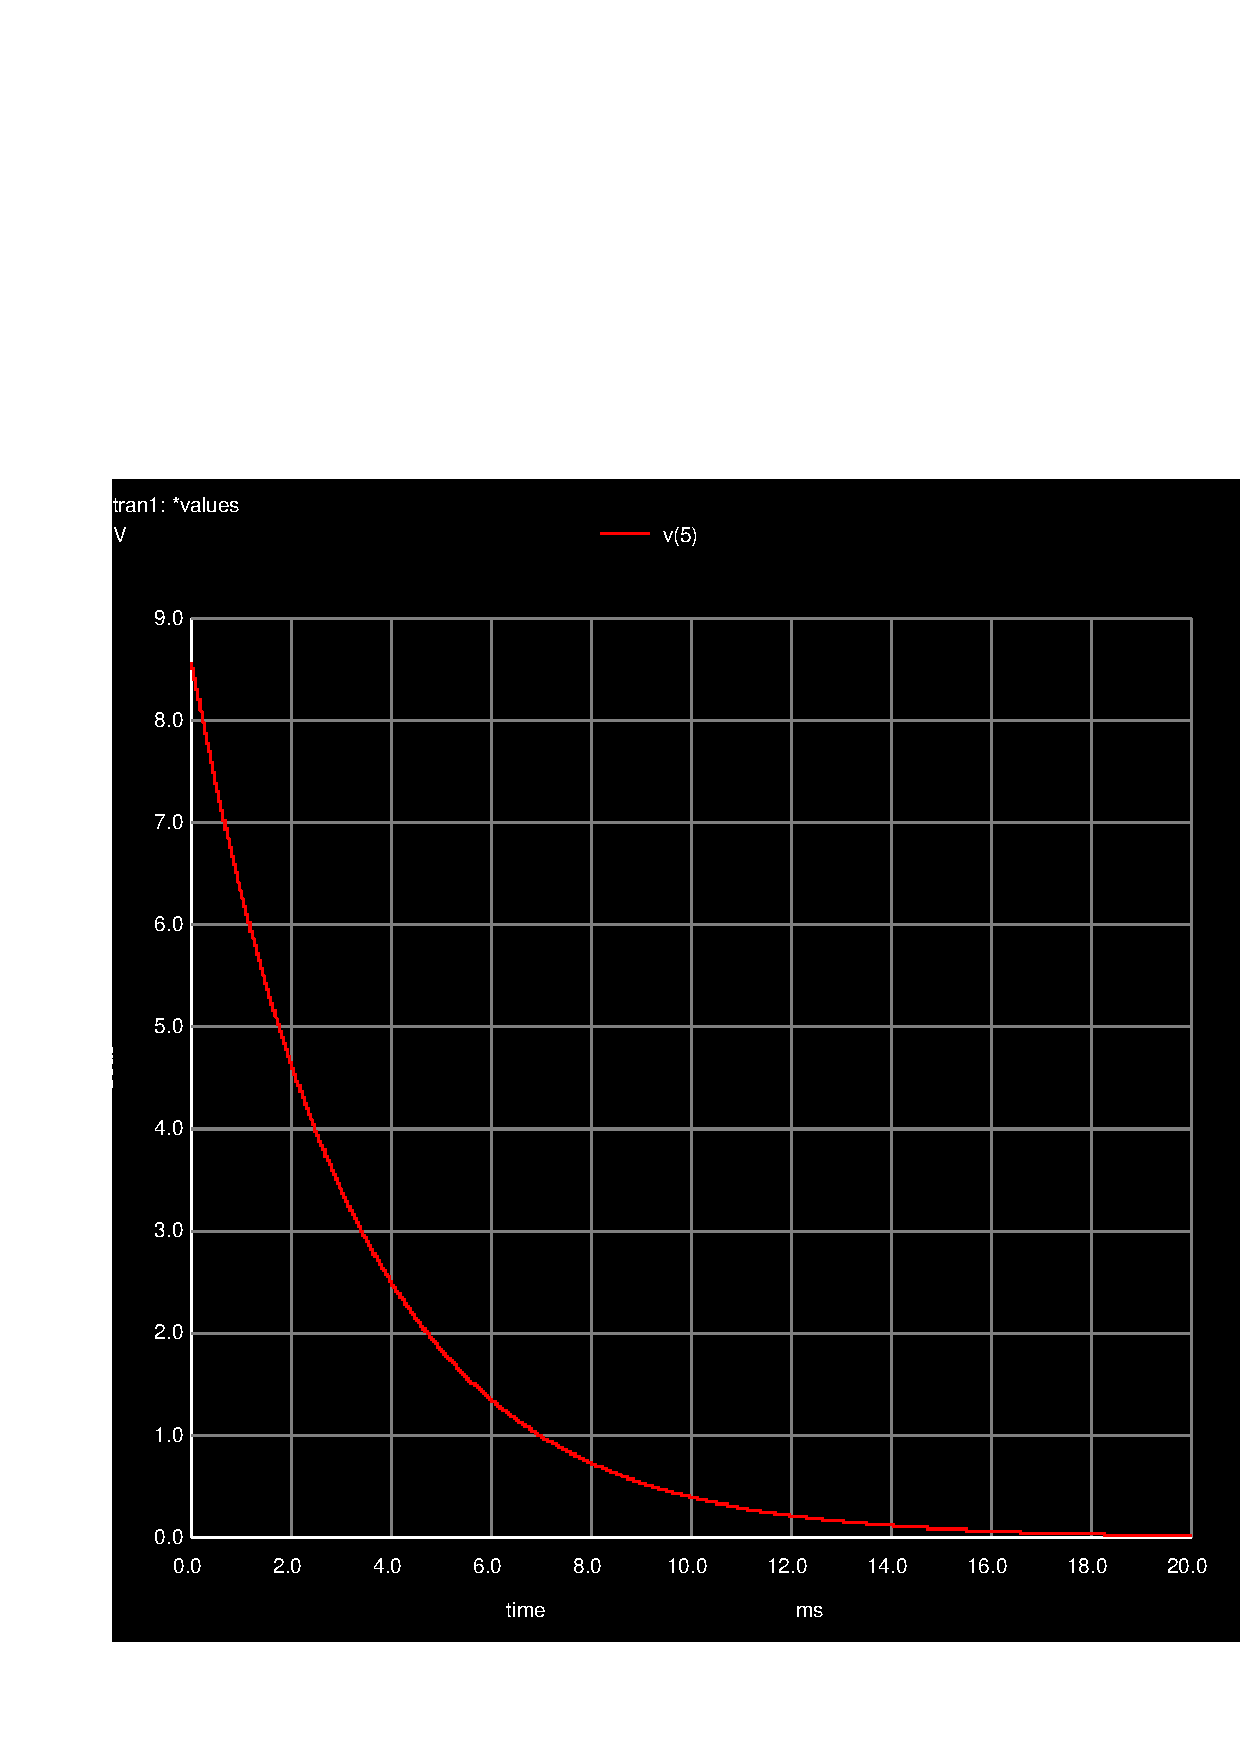
\includegraphics[width=0.6\linewidth]{transv5n.pdf}
\caption{Natural solution for $v_5$}
\label{fig:v5_ng}
\end{figure}
\FloatBarrier

\subsection{Natural and forced responses for f = 1kHz and given $v_S$(t)}

The plot for $v_S$(t) and the circuit's response can be seen in \ref{fig:transv5vs.pdf}.

\begin{figure}[h] \centering
\includegraphics[width=0.6\linewidth]{transv5vs.pdf}
\caption{Stimulus (blue) and response (red) on node 5}
\label{fig:transv5vs.pdf}
\end{figure}
\FloatBarrier


\subsection{Frequency response}

For f$\in$[0.1Hz;1MHz] the frequency response in node 5 is simulated. The functions $v_S$(f) and $v_5$(f) are plotted in a logarithmic scale (dB) in \ref{fig:db_v5_v1.pdf}, and the phases can be seen in degrees in \ref{fig:phase.pdf}. 
%EXPLICAR

\begin{figure}[h] \centering
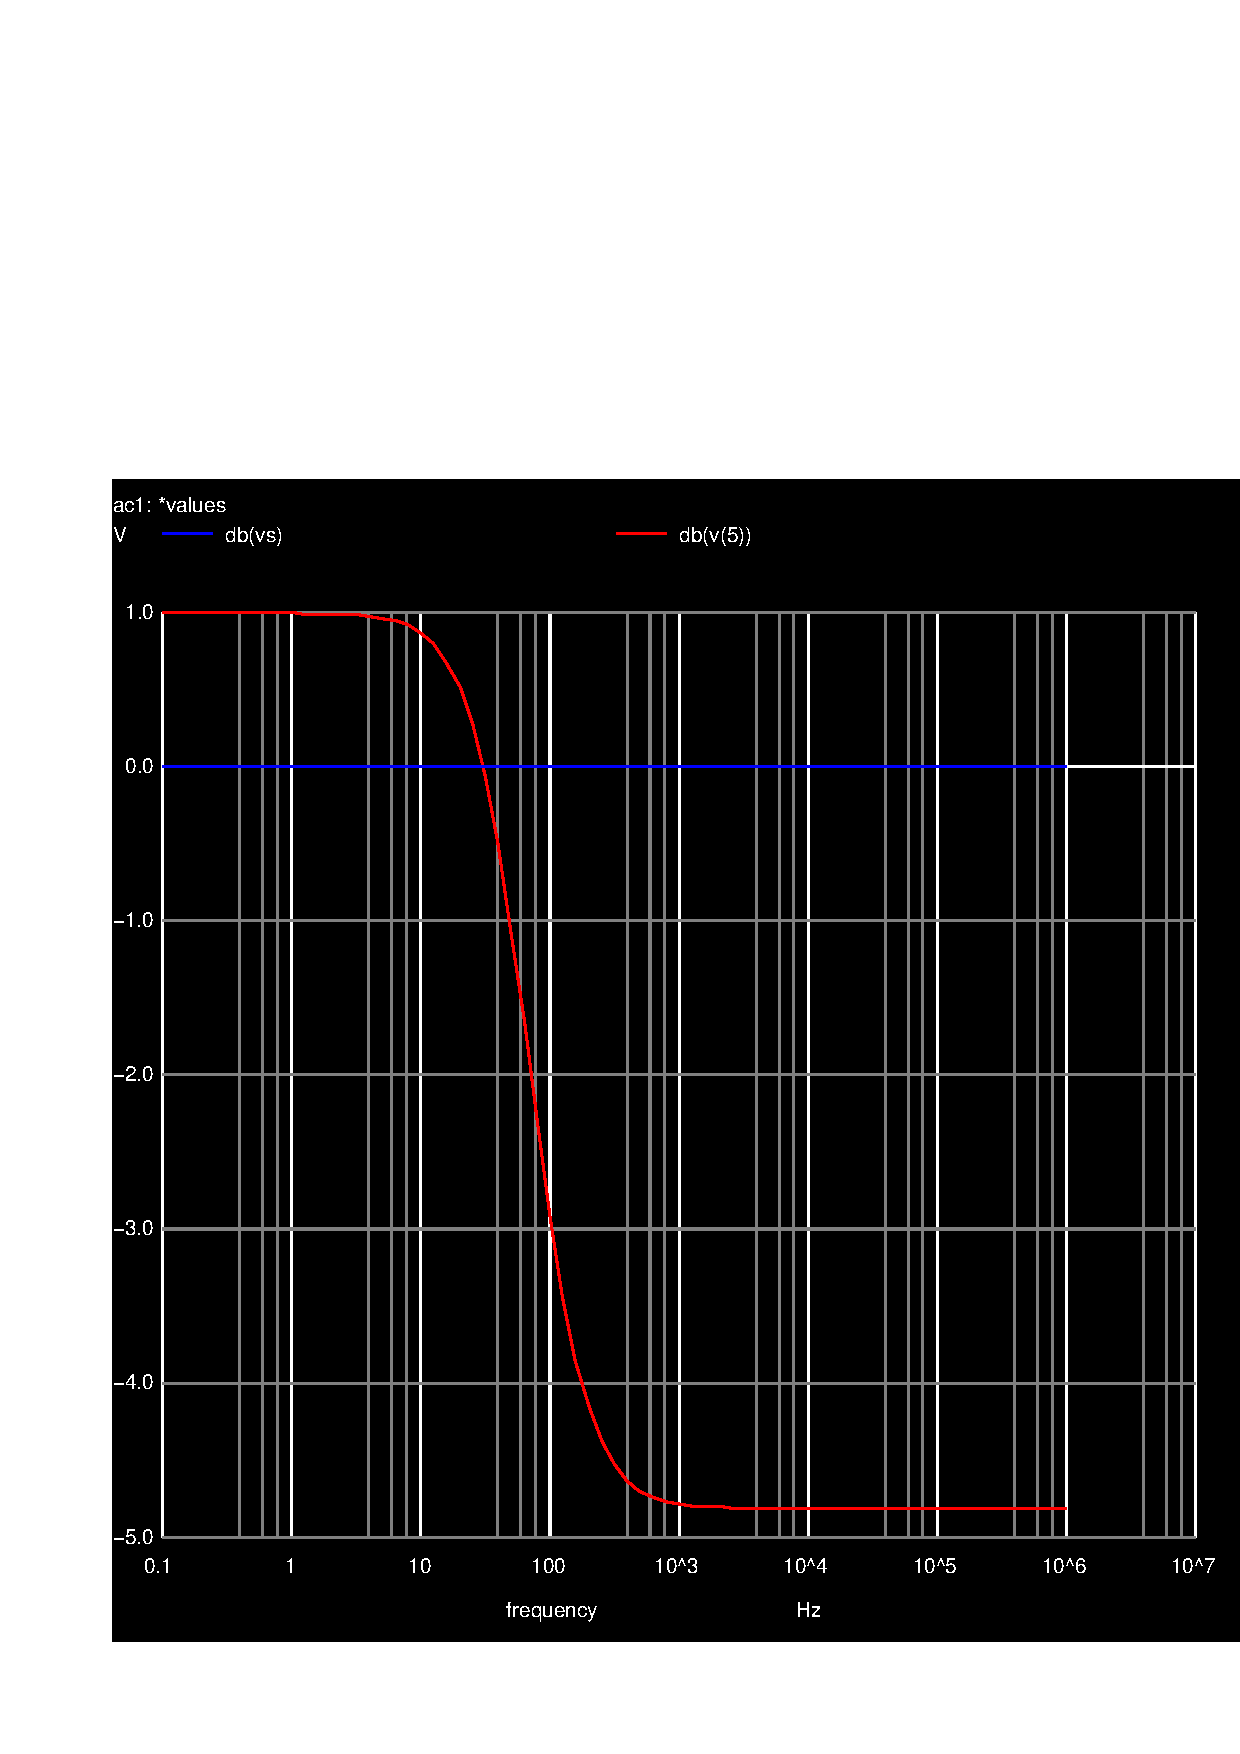
\includegraphics[width=0.6\linewidth]{db_v5_v1.pdf}
\caption{$v_S$(f), in blue, $v_5$(f), in red, and $v_C$(f), in yellow}
\label{fig:db_v5_v1.pdf}
\end{figure}
\FloatBarrier

\begin{figure}[h] \centering
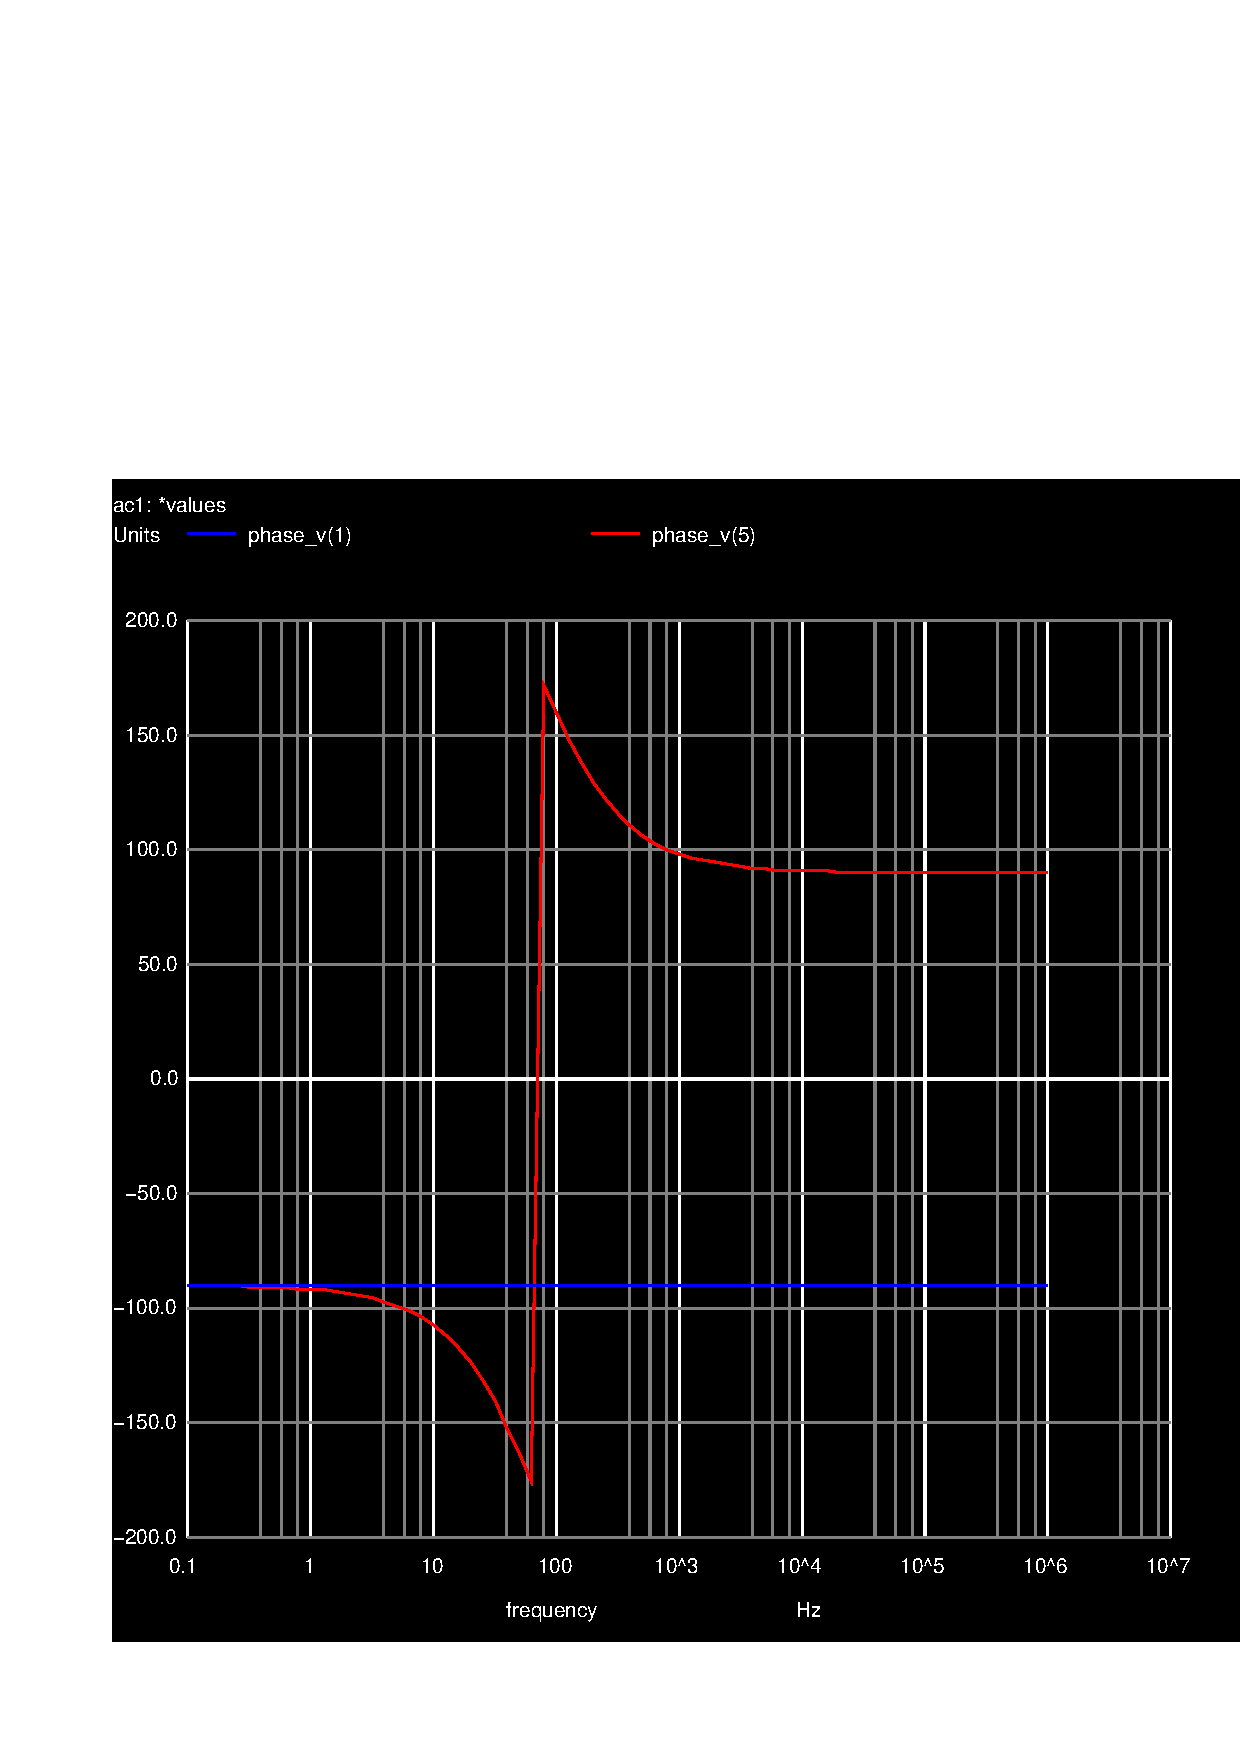
\includegraphics[width=0.6\linewidth]{phase.pdf}
\caption{Phase of $v_S$(f), in blue, $v_5$(f), in red, and $v_C$(f), in yellow}
\label{fig:phase.pdf}
\end{figure}
\FloatBarrier
